\section{System Design} \label{sec:system}

\begin{figure}[t]
\centering
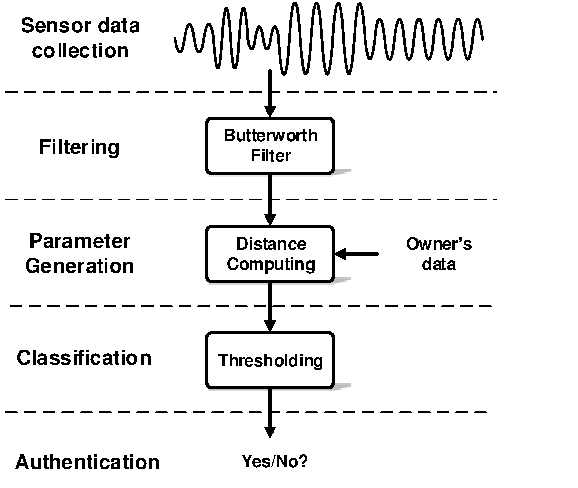
\includegraphics[width=0.75\columnwidth]{pic/system.eps}

\caption{\systemname~system design flow. The online authentication phase of \systemname~consists of the following steps: (1) sensor data collection in which we collect accelerometer data while users move their head as a response to an audio track played on the glass, (2) filtering in which we apply a Butterworth filtering to smoothen the sensor data for subsequent processing, (3) parameter generation in which we calculate the distances between two accelerometer samples as the parameter, and (4) classification in which we adopt an adaptive thresholding mechanism to classify the user's head movement, whose output will be used as the authentication result.}
\label{fig:sysarch}
\end{figure}


We design the \systemname~ system as a software service that provides direct authentication for users through their head--movements, to login to their smart--glass devices and authenticating to the apps running on the device. We envision that \systemname~will execute upon device power--up or wake--up or application initiation; a mechanism that is similar to that of screen unlocking in smartphones.
In~\systemname the authentication process is divided into two steps: a training phase and an online authentication phase. In the training phase, the system collects accelerometer data corresponding to the user's head movements stimulated through music cues for a specific duration, and uses the data samples to build a binary classifier. For simplicity, in our current implementation we execute the training--phase off--line. In reality, the training data would be accumulated over time to keep the system up-to-date. Extending the implementation towards on--line training will only require minor modifications to the software modules in our current implementation. In the online authentication phase, the user performs the same head movement (as in the training phase) under the same music cue settings and attempt to authenticate to the device. \systemname~ modules collect the samples and labels them based on the local training data--base and the online classifier output. The user is authenticated to the device if the output from the binary classifier is \textit{successful}, and not \textit{failed}.

As shown as Fig.~\ref{fig:sysarch}, the authentication process in \systemname~ involves four key components: sensing, filtering, distance computing and classification. We briefly discuss these system design components in the following subsections.

\subsection{Sensing and Filtering}
The sensing step involves collecting data samples from the built--in accelerometer when the user performs head--movements, in response to the given music cue with duration of $T$ seconds. The raw sensor data is collected from 3 axis at a sampling rate of $r$ points/sec. Thus, each sample is a matrix of $3 \times rT$ points. $T$ is set to be in the order of few seconds, considering the fact that frequency of human movements are in that order.
A low--pass Butterworth filter~\cite{challis1983design}, using a cut--off frequency of 10 Hz, then removes high frequency noise from the sensor raw data.

\subsection{Distance Computing}
This step is the preparation stage for a binary classifier. We adopt a simple technique for distance computation, through Dynamic Time Warping (DTW)~\cite{dtw}, as it is feasible to implement the same even on computing resource--constrained wearable device. We use the DTW distance in our implementation. Let us suppose that there are two time series samples $S_a = (s_1,s_2, ... ,s_n)$ and $S_b = (s_1, s_2, ..., s_n)$. The DTW distance is defined as the temporal separation between  the samples when the optimal alignment between $S_a$ and $S_b$ has been determined by time--warping the two series in a non--linear fashion~\cite{dtw}.

\subsection{Classification}
The classification phase determines a test sample as \textit{successful} or \textit{failed} based on a threshold. Thresholding--based classifier strikes a good balance between simplicity and good performance. 

For the training phase, we design a technique for choosing $Top-K$ template samples from the whole training set. We compute an average distance for each sample by computing the DTW distance of each sample to all other samples. The top $K$ samples with the smallest average distance are chosen as templates. These $K$ samples represent the sample space, as they are essentially an empirical estimation of the centroid of the data sample space. In the classifier, only the $Top-K$ samples are contained thus reducing the computation load and adding robustness against randomness of the samples in the system. We establish a threshold for the each of the $Top-K$ samples. It is determined by average value of the distance, $\mu_s$, and the standard deviation, $\sigma_s$. The threshold is defined as $\mu_s + n\sigma_s$, where $n$ is a tunable parameter in the classifier, and can take real positive number values. 

In the online authentication phase, if the DTW distance between the test sample and the template is below the threshold for the chosen template, we label the test sample as {\em successful}, otherwise as {\em failed}. Since an classification output if obtained for each of the $Top-k$ samples, we chose the sample based on a voting strategy that choses based on majority.
%Among three steps outlined above, the first two steps belong to the training phase and the third step belongs to the online authentication phase. 
Eventually, if the user's test data is classified as {\em successful} the user is accepted (authenticated for login) by the system; otherwise, the user is rejected. 



     